\emph{Browsershots} fornisce un'interfaccia che permette di testare, dato un indirizzo web, un qualsiasi sito in una miriade di browser 
e sistemi operativi diversi.\\
Lo strumento ci è stato molto utile per provare la stabilità della struttura del sito in qualunque ambiente. 

\begin{figure}[!h]
	\centering
	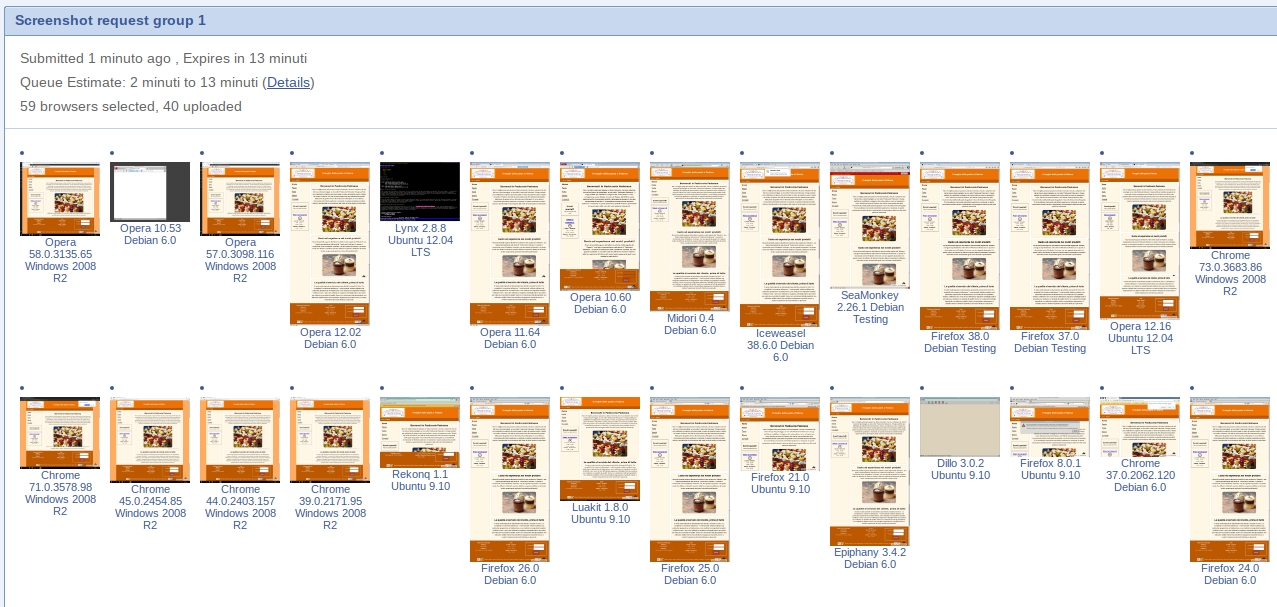
\includegraphics[width=0.7\linewidth]{sezioni/FaseTest/Immagini/browsershots.png}\\
	\caption{Browsershots – browser tester}
	\label{Fig:browsershots}
\end{figure} 
\newpage